\section{Program flowchart}
\label{chapter3}


\paragraph{}
Figure \ref{fig:stateDiagrams} shows the state transition diagrams for Node 1 and Node 2. Both nodes execute a thread that sets up the Bluetooth communication and sends and receives data. Node 1 executes a second thread which periodically fetches the proximity sensor readings, and provides them to the communication thread for transmission to Node 2. Node 2 executes a thread which uses the current speed and distance data to automatically control the vehicle speed if the ACC system is turned on.

\begin{figure}[h]
	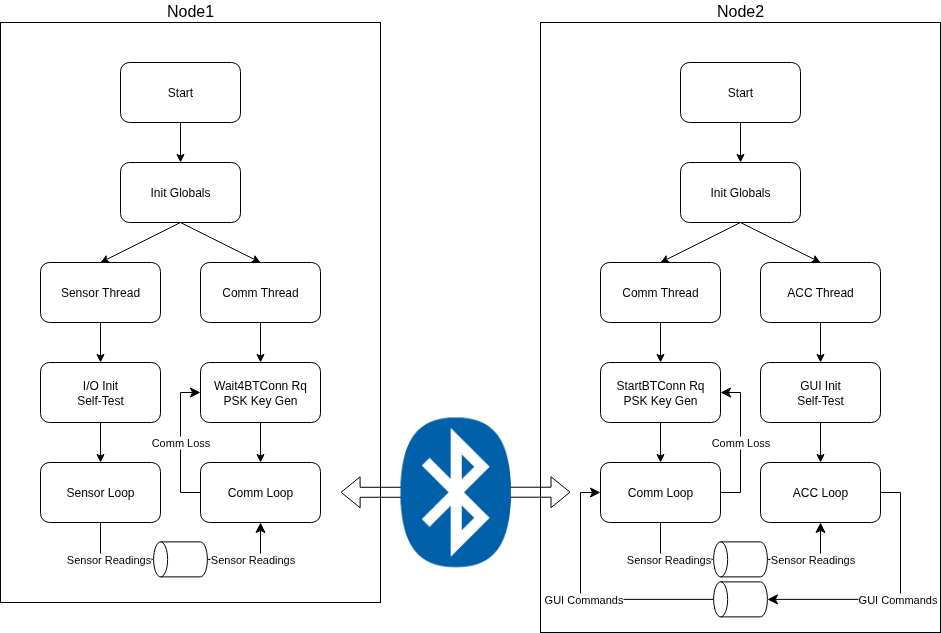
\includegraphics[height=100mm]{images/StateDiagrams.png}
	\centering
	\caption{State Diagrams}
	\label{fig:stateDiagrams}
\end{figure}

\paragraph{}
Figure \ref{fig:stateDiagramNode1} shows the two thread loops of Node 1 in more detail. The Sensor Loop sequentially obtains readings from one of the two connected sensors, checks the value for plausibility and consistency with previous readings. Depending on whether values are OK, the thread pushes the normalized distance data or an error code to a global variable, where the communication thread picks it up for further transmission. In the end, the thread switches the sensor to read from and puts itself to sleep for 50ms, after which it starts over.

\paragraph{}
In the communication loop the thread picks up the distance data from a global variable and puts it into a sensor message which it protects with a MAC and transmits to Node 2. If the transmission fails, the Bluetooth connection is closed and a new one is set up. On successful transmission, the thread puts itself to sleep for 25ms after which it starts over.

\paragraph{}
The steps in Figures \ref{fig:stateDiagramNode1} and \ref{fig:stateDiagramNode2} which are drawn in inverted color involve read or write operations on shared global data. In order to avoid race conditions the read/write operations are protected in critical sections.

\begin{figure}[h]
	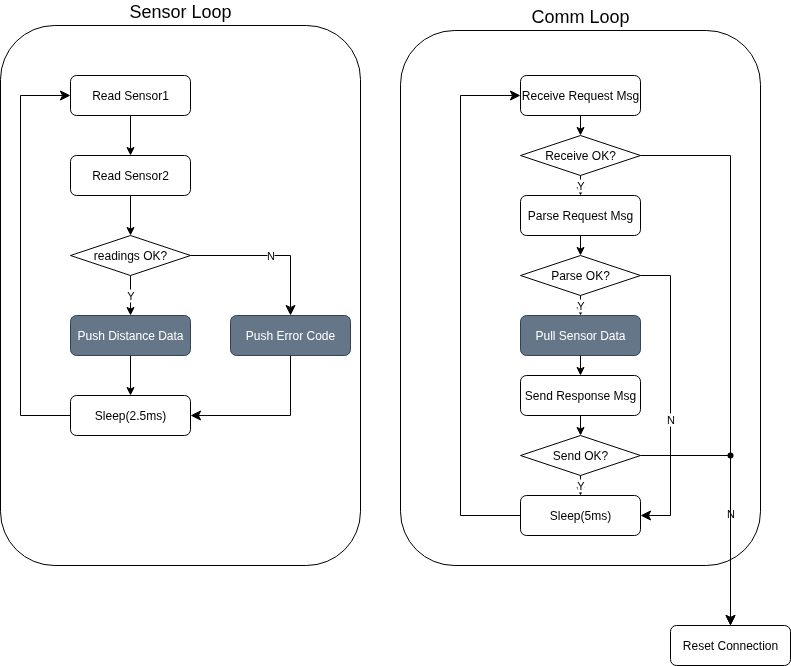
\includegraphics[height=100mm]{images/StateDiagramNode1.png}
	\centering
	\caption{State Diagrams Node 1}
	\label{fig:stateDiagramNode1}
\end{figure}

\paragraph{}
Figure \ref{fig:stateDiagramNode2} shows the two thread loops that execute on Node 2. The communication loop receives the sensor message synchronously (i.e. the call blocks until a message is received). After reception, it verifies the MAC of the received message and parses the payload of the message. If both steps were successful, the received sensor data is copied into a global variable, together with the current timestamp, where it can be picked up from the ACC thread. If the reception fails,
the thread closes the Bluetooth connection and tries to set up a new one. In the case that the reception was successful, but MAC verification or message parsing were failing, the received message is ignored. In the end, the thread starts over by receiving the next message.

\paragraph{}
The ACC loop retrieves from the GUI the ACC status (whether the driver has turned it on or off) and, if it is turned off, the current, manually set, speed. In the next step, it obtains the Sensor data (i.e. the most recently received distance data). If the received data contains a valid reading, it updates its local copies of the last valid reading and the timestamp. If the state of the ACC was the ERROR state, it is reset to the OK state. In the next step, the thread verifies that the timestamp of its last valid reading is not older than 500ms. If the timestamp is older, the state of the ACC is set to ERROR.
In the next step, if ACC is in the ON state, a control function \emph{Speed = ACC(Distance, Speed)} is applied, i.e. the ACC accelerates/decelerates the car depending on the current vehicle speed and measured distance.
Thereafter, the current vehicle speed, distance, and ACC state is conveyed to the display so it can update the corresponding GUI elements. Finally, the control loop puts itself to sleep for 50ms and thereafter starts over. Like in the previous diagram, steps in inverted color indicate read/write accesses to data shared across threads. These accesses are protected by critical sections.

\begin{figure}[h]
	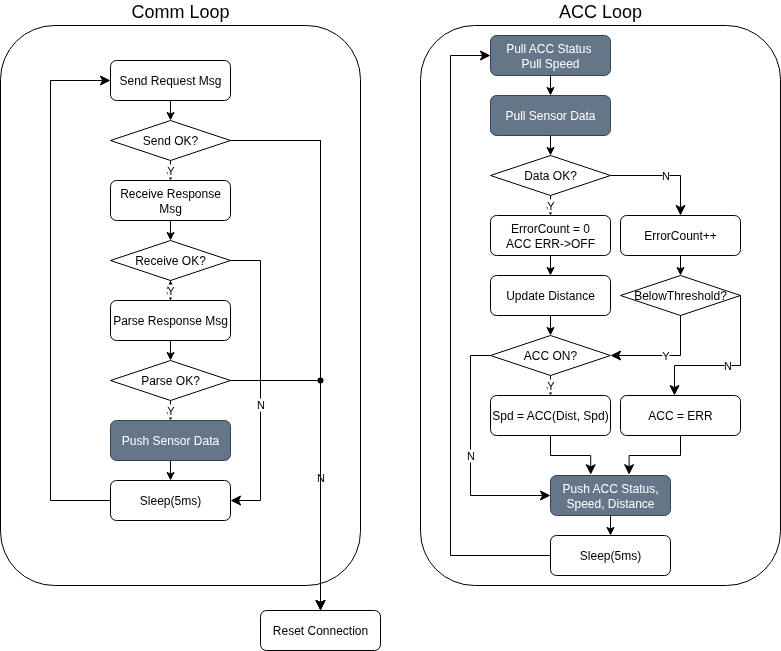
\includegraphics[height=100mm]{images/StateDiagramNode2.png}
	\centering
	\caption{State Diagrams Node 2}
	\label{fig:stateDiagramNode2}
\end{figure}
